\section{Dormant Attention Heads}\label{sec:dormant_heads}
 
 In this section, we will more carefully define dormant heads and show that they are ubiquitous on both pre-trained LLMs and small transformers trained via next-token-prediction.

\subsection{Dormant Head Conjecture} \label{sub:dormant_head_conjecture}

As in \Cref{sub:case_study_l25_h16}, we define a \textit{dormant attention head} as follows.
\begin{quote}
    \textit{An attention head is \underline{dormant} on a particular input if its output consists of only one (or a small number of) vector(s), repeated across every token index.}
\end{quote}
 The output of a dormant head does not respect the semantic content of the input, and essentially outputs a bias. Heads which are attention sinks are dormant attention heads, and indeed almost all (but not necessarily all) dormant attention heads are attention sinks. Our \textit{dormant heads conjecture} states that dormant heads are ubiquitous in LLMs. In particular, we say that a head which is not dormant is \textit{active}. Then, we conjecture the following:
 \begin{quote}
     \textit{\underline{Dormant heads conjecture:} for autoregressive transformer-based language models, a large fraction of heads are dormant on some inputs and active on some others.}
 \end{quote}
 In this section, we will provide evidence for this conjecture through finding a circuit in Llama 2 7B which creates dormant heads (\Cref{sub:circuit_evidence}), developing an automated detection system for attention sinks and thus showing that many heads in Llama 2 7B are empirically dormant on some inputs and active on others (\Cref{sub:lots_of_dormant_heads}), and showing that the dormant head phenomenon persists in small autoregressive transformers trained on next-token-prediction (\Cref{sub:controlled_experiments}).

\DP{TODO: description}

\subsection{Evidence 1 For Conjecture: Circuit for Dormant Heads in Llama 2} \label{sub:circuit_evidence}

\DP{TODO: description}

\begin{figure}[t]
  \centering
  % \begin{minipage}{0.24\textwidth}
  %     \centering
  %     \subcaption{\small Attention weights}
  %     \label{fig:circuit-attn-weights}
  %     \vspace{-.2em}
  %     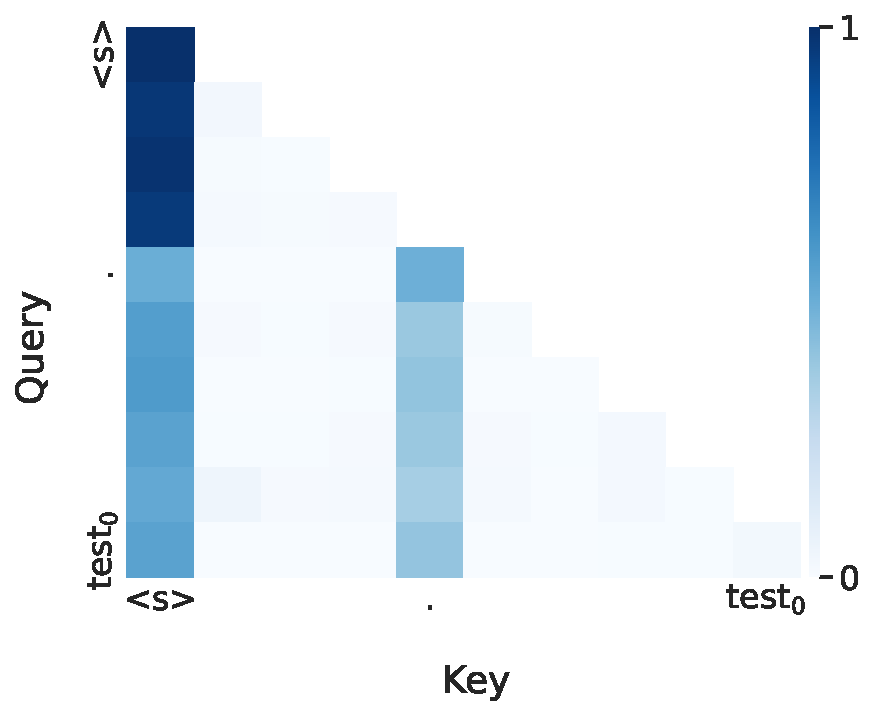
\includegraphics[width=\linewidth]{Figures/figures_circuit/attn_weights_dormant.pdf}
  % \end{minipage}
  % \hspace{-1em}
  \begin{minipage}{0.33\textwidth}
      \centering
      \subcaption{\small Attention logits}
      \label{fig:circuit-attn-logits}
      \vspace{-.2em}
      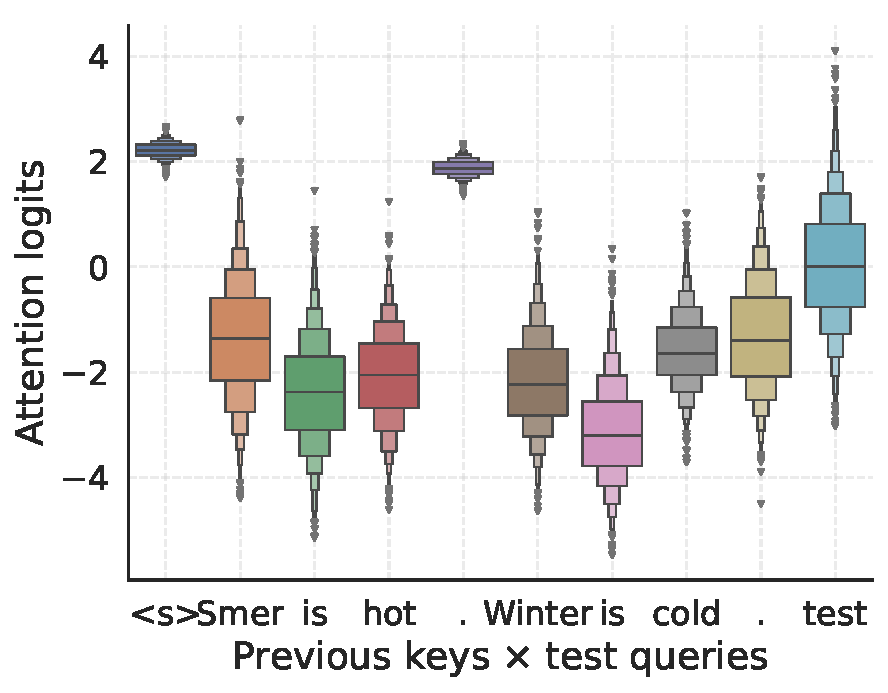
\includegraphics[width=\linewidth]{Figures/figures_circuit/logits.pdf}
  \end{minipage}~
  % \hspace{-1em}
  \begin{minipage}{0.33\textwidth}
      \centering
      \subcaption{\small Output norm}
      \label{fig:circuit-massive-norm}
      \vspace{-.2em}
      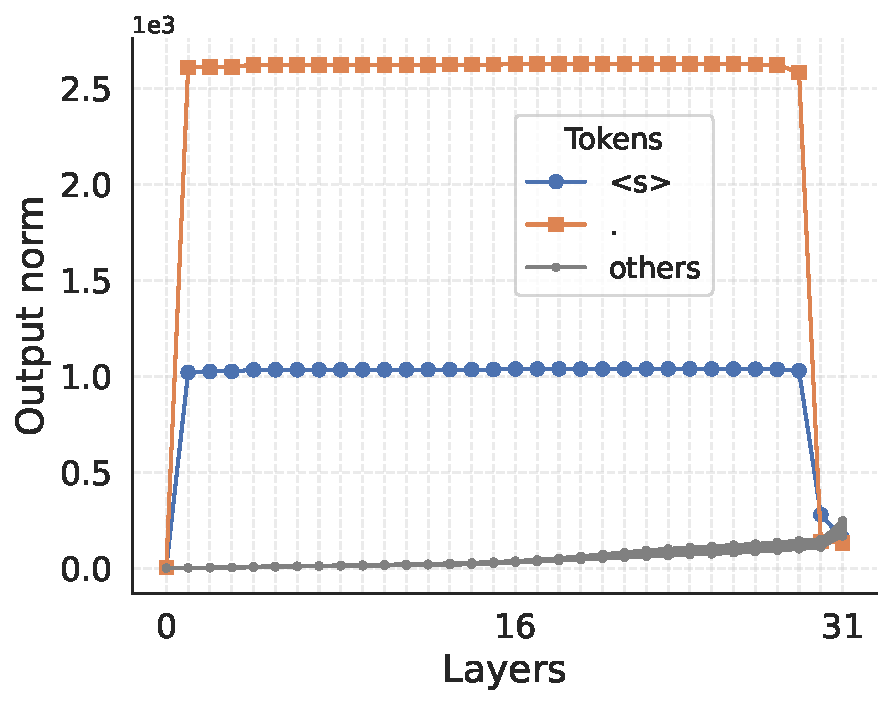
\includegraphics[width=\linewidth]{Figures/figures_circuit/massive.pdf}
  \end{minipage}
  \hspace{-1em}
  \begin{minipage}{0.33\textwidth}
      \centering
      \subcaption{\small Value states norm}
      \label{fig:circuit-value-norm}
      \vspace{-.2em}
      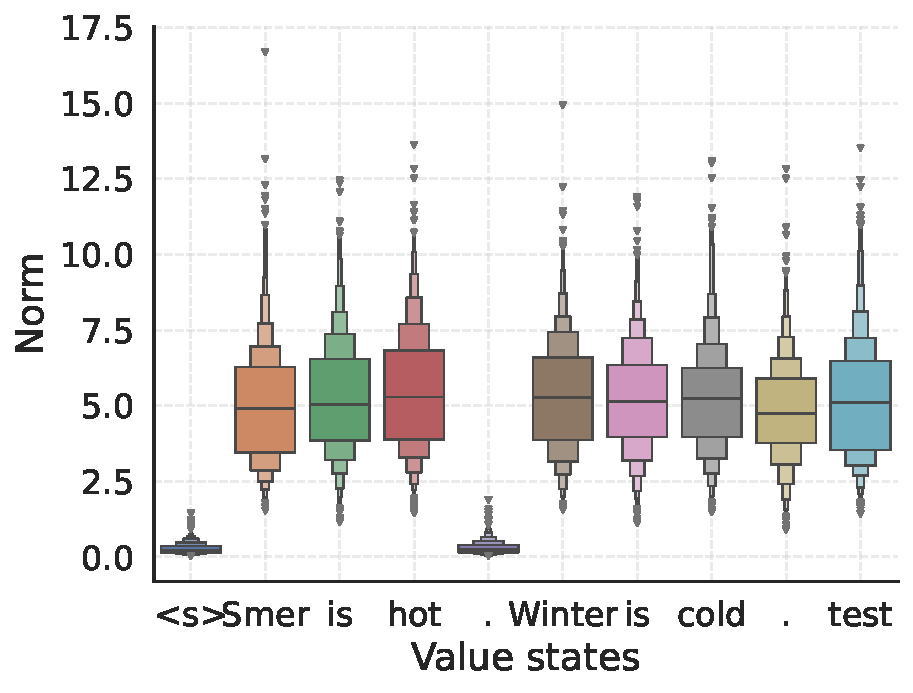
\includegraphics[width=\linewidth]{Figures/figures_circuit/values.pdf}
  \end{minipage}
  \vspace{-1em}
  \caption{\small \textit{Algebraic findings.} We sample ``\bos~Summer is hot. Winter is cold.'' $+$ ``random test token'''s for $1000$ times to obtain a distribution of hidden states in \llama. Figure \ref{fig:circuit-attn-logits} presents the attention logits computed by using the test tokens as queries and the previous tokens as keys. The logits on \bos~and the first \delim are effectively positive constants, with logits on other tokens vary among different test tokens, and being mostly negative. Figure \ref{fig:circuit-massive-norm} shows the norm of the outputs across all the layers, with the \bos~and the first \delim possessing significantly massive norms from layers 2 to 29. Figure \ref{fig:circuit-value-norm} shows the norm distribution of the value states across layers 2 to 29. The norms of the \bos~and the first \delim token are effectively small constants. 
  }
  \label{figure:algebra-findings}
  \vspace{-1em}
\end{figure}



We summarize the algebraic features of \bos~ and the first \delim tokens in the computation graph, all of which point to the dormant heads conjecture. Previous works discover parts of these features separately. As a demonstration, we randomly sample 1000 tokens from the vocabulary of \llama, prefix it with ``\bos~Summer is hot. Winter is cold.'' to form one test sequence, and implement the forward pass. By collecting  hidden states for each test sequence, it provides us with a distribution of hidden states.
\ref{figure:algebra-findings} summarizes the four algebraic features:
\begin{enumerate}
    \item \textit{Attention sink}: Figure XXX visualizes the attention weights. Before the first \delim, the attention weights from all tokens on \bos~are near 1. The \delim would split half of the attention weights on \bos.
    \item \textit{Stable attention logits}: Figure \ref{fig:circuit-attn-logits} presents the attention logits from the test token (query) on tokens in the prefix (key). The distribution comes from a fixed head, L16H25, with 1000 test tokens. The attention logits on \bos~and \delim are nearly constant across all test tokens, while vary a lot on other tokens. 
    \item \textit{Massive norms}: Figure \ref{fig:circuit-massive-norm} presents the norm of hidden states across layer 0 to 31, averaged among 1000 test sequences. The \bos~and \delim have norms around 500 to 1000 times of other tokens.
    \item \textit{Small value states}: Figure \ref{fig:circuit-value-norm} shows the norm distribution of norms of value states. The distribution comes from all heads from layer 2 to 29 and with 1000 test tokens. \bos~and the first \delim both possess negligible norm.
\end{enumerate}

\tianyu{I will postpone the circuit here}
The algebraic findings depict a potential circuit of the dormant mechanism. Figure XXX illustrates the entire procedure, which we summarize as follows:
\begin{enumerate}
    \item Preparatory phase (layer 0 and 1): The $\mlp$ of layer 1 adds an output with massive norm residual streams of \bos~and the first \delim tokens. Using causal ablations, we verify the function of each components in layer 0 and 1.
    \begin{enumerate}
        \item \tianyu{We need to discuss the names here} Both the $\MLP$ in layer 0 and 1 contribute to the formation of a XXX in layer 1.
        \item $\Attn$ in both layer 0 and 1 adjust the formation of XXX. For example, shown by zero-out intervention, L1H8 both assists the initial token to be XXX and suppresses the other tokens to be XXX.
        \item The \rope in $\Attn$ heads in layer 0 and 1 suppresses the formation of XXX starting from the second delimiter tokens.
    \end{enumerate}
    \item Dormant/active phase: At this stage, the residual streams of \bos~and the first \delim remain nearly untouched, since any outputs added on the residual stream have negligible norms. At the main time, the layer norm map them to a special direction XXX, which corresponds to a sink key state which has nearly constant attention logits fitted with any queries. The direction XXX also possesses minor value states,. As a result, a test token has two modes on the attention weights:
    \begin{itemize}
        \item dormant mode: when no other keys align with its queries. After the Softmax function, \bos~and the first \delim take up a great proportion of its attention weights
        \item active mode: when there's other key that aligns with its query, which renders a attention logits comparable or even greater than the attention logits on \bos. After the Softmax function, \bos~and the first \delim take up a small proportion of its attention weights.
    \end{itemize}
    Since the value states of \bos~and \delim are notably small,
    The different modes on attention weights lead to different     \begin{itemize}
        \item dormant mode: add a minor output on the residual stream
        \item active mode: add a large output on the residual stream
    \end{itemize}
\item Recover phase: On \bos~and \delim, the $\MLP$ in the last two layers add a massive norm on the residual, while on its negative direction. As a result, The norms of \bos~and \delim become normal. There's no dormant phenomenon in last two layers.
\end{enumerate}

After the preparatory work in layers $0$ and $1$, the


\subsection{Evidence 2 For Conjecture: Abundance of Dormant Heads in Llama 2} \label{sub:lots_of_dormant_heads}

\DP{TODO: description}

\subsection{Evidence 3 For Conjecture: Dormant Heads in Small Transformers} \label{sub:controlled_experiments}

We further demonstrate that attention heads learn to be dormant even under a toy task, which we call as the \textit{dormant copy} task. As illustrated in Figure \ref{fig:pretraining-dgp}, we generate the input sequence with three steps. First, we always start with a \bos~token. Second, on normal tokens, we use a pre-determined Markov transition probability $P_e$ to predict the next token. Third, on $k$ trigger tokens, instead of using the Markov transition $P_e$, we copy the previous token to the next position. Similar to \citet{bietti2024birth}, we choose the $P_e$ and the vocabulary from the estimated character-level bigram distribution on the tiny \textit{Shakespeare} dataset. We manually add the \bos~token to the character-level vocabulary of \textit{Shakesphere}, making it to contain $N_{voc}=66$ tokens in total. 
To avoid repeat occurrence of the \bos~token, We sample the second token from the estimated unigram distribution in the \textit{Shakespeare} dataset, but drop the sequence if it's a trigger token. We fix the trigger tokens as the $k=3$ most frequent tokens in the unigram distribution.

The optimal algorithm for the \textit{dormant copy} task is to predict the next token distribution with $P_e$ on normal tokens and with previous tokens on trigger tokens. The transformer structure allows it to replicate the optimal algorithm. With the dormant conjecture in mind, since normal tokens do not require any in-context mechanism, we expect the $\Attn$ layer is dormant with only the $\MLP$ layer takes effect. The trigger tokens require the copying from the previous token, on which we expect the $\Attn$ layer is active. 

To verify our dormant/active modes mechanism, we pre-train a transformer with $1$ layer and $1$ head on the \textit{dormant copy} task using ADAM for $10000$ rounds. The resulting transformer could match the optimal algorithm on the prediction loss. More importantly, we observe clear patterns of the $\Attn$ head being dormant or active. Figures \ref{fig:pretraining-attn-weights-dormant} and \ref{fig:pretraining-attn-weights-active} visualize the attention weights on different input sequences. Figure \ref{fig:pretraining-attn-weights-dormant} shows that the \Attn head is dormant, with all attention weights are on the \bos~token when there's no trigger token. As a result, the \Attn head only adds a constant to the residual stream of normal tokens. Figure \ref{fig:pretraining-attn-weights-active} shows that the \Attn head is active and attend on the previous tokens from trigger tokens, which adds information from the previous tokens on the residual stream of trigger tokens.

\begin{figure}[t]
  \centering
  \begin{minipage}{0.4\textwidth}
      \centering
      \subcaption{\small Data generating procedure}
      \label{fig:pretraining-dgp}
      \vspace{-.2em}
      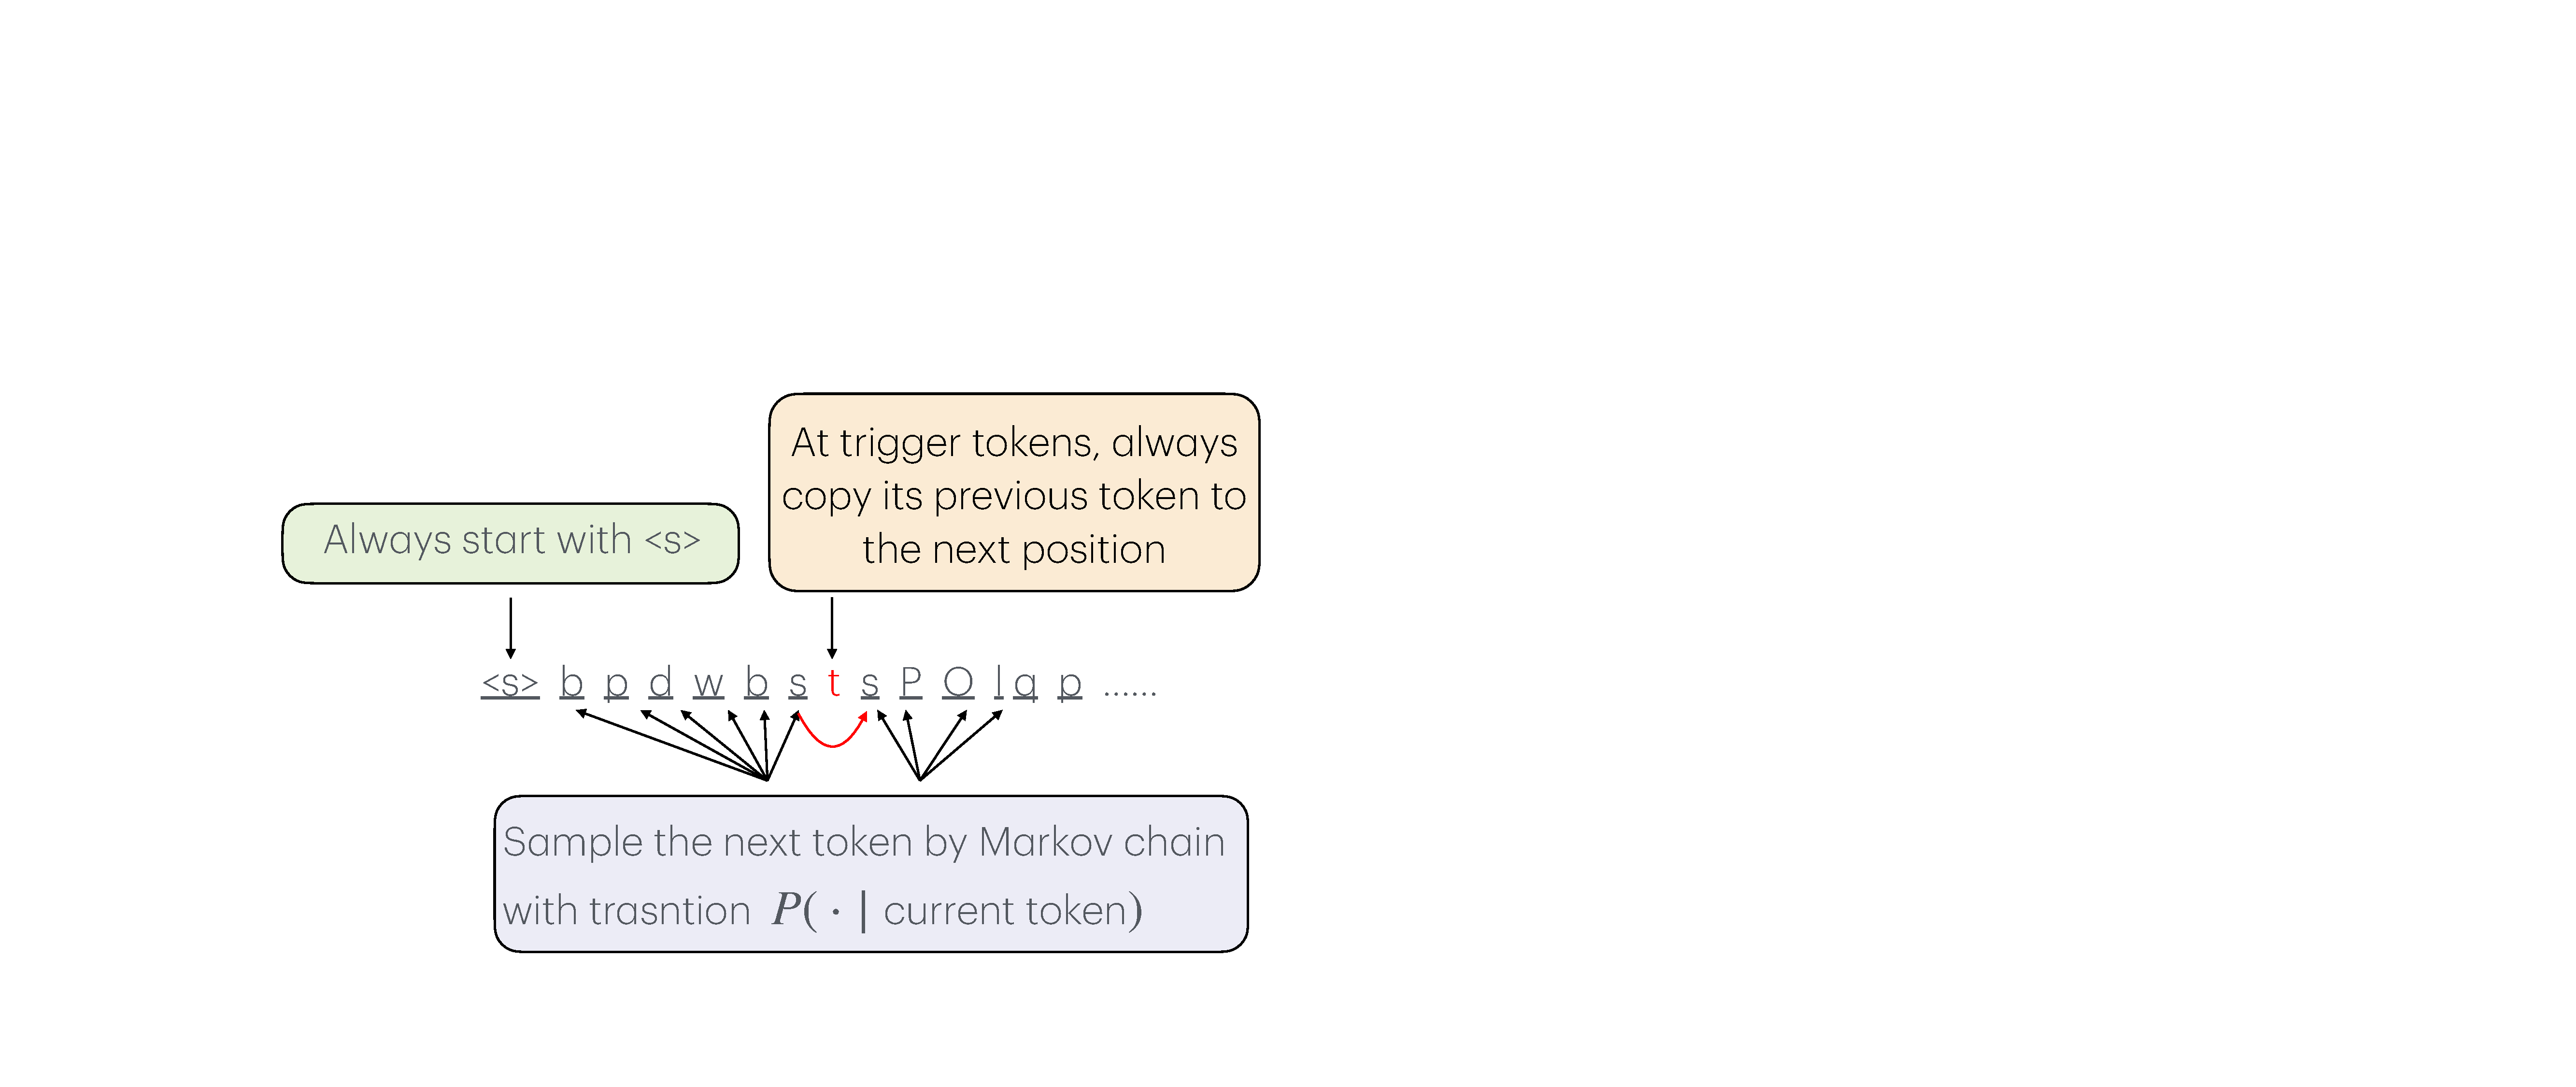
\includegraphics[width=\linewidth]{Figures/figures_pretraining/dormant_copy.pdf}
  \end{minipage}
  \hspace{-1em}
  \begin{minipage}{0.3\textwidth}
      \centering
      \subcaption{\small Dormant}
      \label{fig:pretraining-attn-weights-dormant}
      \vspace{-.2em}
      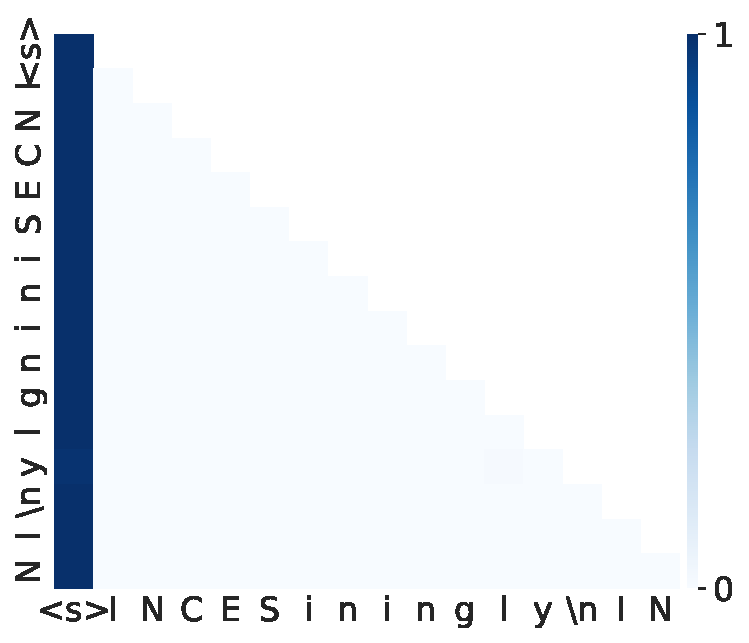
\includegraphics[width=\linewidth]{Figures/figures_pretraining/dormant_copy/dormant_copy_attn_weights_seq0.pdf}
  \end{minipage}
  \hspace{-1em}
  \begin{minipage}{0.3\textwidth}
      \centering
      \subcaption{\small Active}
      \label{fig:pretraining-attn-weights-active}
      \vspace{-.2em}
      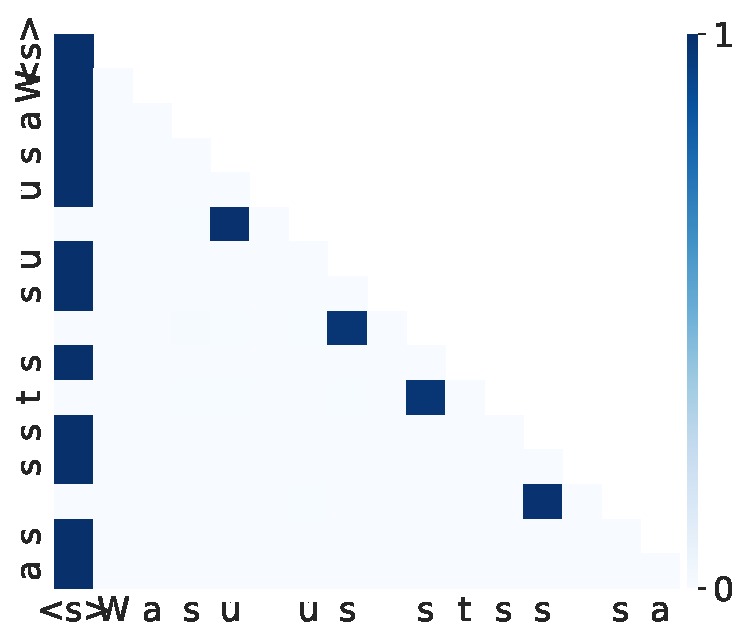
\includegraphics[width=\linewidth]{Figures/figures_pretraining/dormant_copy/dormant_copy_attn_weights_seq1.pdf}
  \end{minipage}
  % \vspace{-1em}
  \caption{\small \textbf{The dormant copy experiment.} Figure \ref{fig:pretraining-dgp} illustrates the data generating procedure of the dormant copy task. We fix `t', `e', and ` ' as three trigger tokens. Figure \ref{fig:pretraining-attn-weights-dormant} shows the attention weights on an input without triggers, with the $x$-axis representing the key tokens and the $y$-axis representing the query tokens. The \bos~token takes up nearly all the attention weights among all tokens. Figure \ref{fig:pretraining-attn-weights-active} shows the attention weights on an input with triggers. The \Attn head still puts all attention weights on normal tokens. However, it is active on trigger tokens and attend to the previous tokens.}
  \label{figure:pretraining-findings}
  \vspace{-1em}
\end{figure}

Moreover, on a pre-trained transformer with $3$ layers, we could recover all the algebraic features of the dormant mechanism in large language models. Figure \ref{fig:pretraining-massive-norm} presents the distribution of output norms of layer $1$ on different tokens, sampled from $512$ input sequences with each has $256$ tokens. The output norm of \bos~(around 100) is notably greater than most tokens. Surprisingly, the token $\backslash n$ has even greater norm. Figure \ref{fig:pretraining-small-value} presents the corresponding distribution of value states. Matching the massive norms of the output, \bos~and $\backslash n$ both possess remarkably small value states. It's unclear why the token $\backslash n$ also exhibits similar features with the \bos~token. We conjecture that similar to the first \delim token in \llama, the $\backslash n$ assists the dormant mechanism with the \bos~token. We delegate attention weights plots supporting this conjecture in the appendix.

\begin{figure}[t]
  \centering
  \begin{minipage}{0.4\textwidth}
      \centering
      \subcaption{\small Massive norms}
      \label{fig:pretraining-massive-norm}
      \vspace{-.2em}
      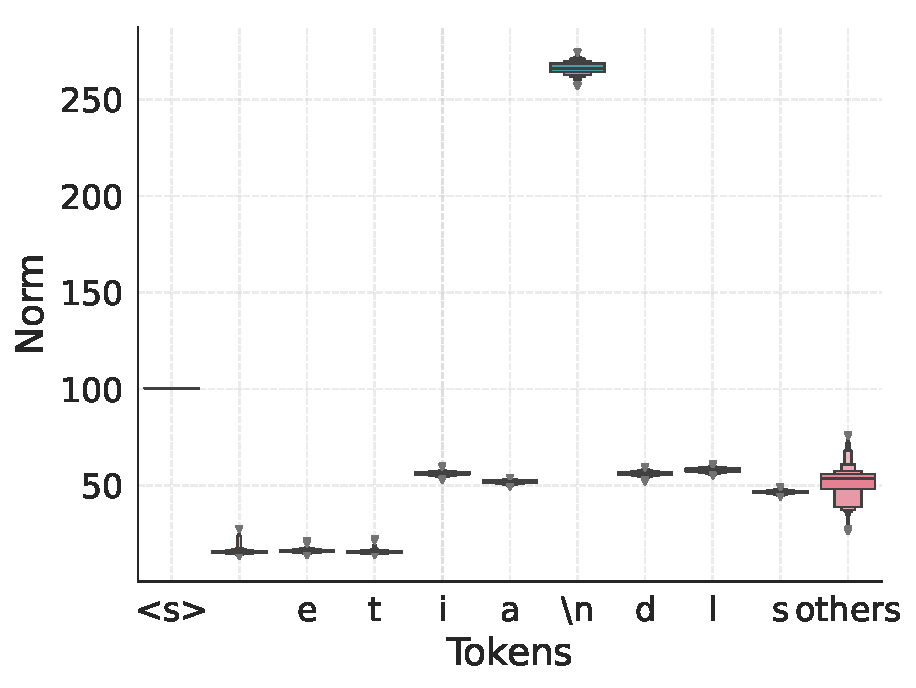
\includegraphics[width=\linewidth]{Figures/figures_pretraining/dormant_copy/dormant_copy_L3_massive.pdf}
  \end{minipage}
  \begin{minipage}{0.4\textwidth}
      \centering
      \subcaption{\small Small value states}
      \label{fig:pretraining-small-value}
      \vspace{-.2em}
      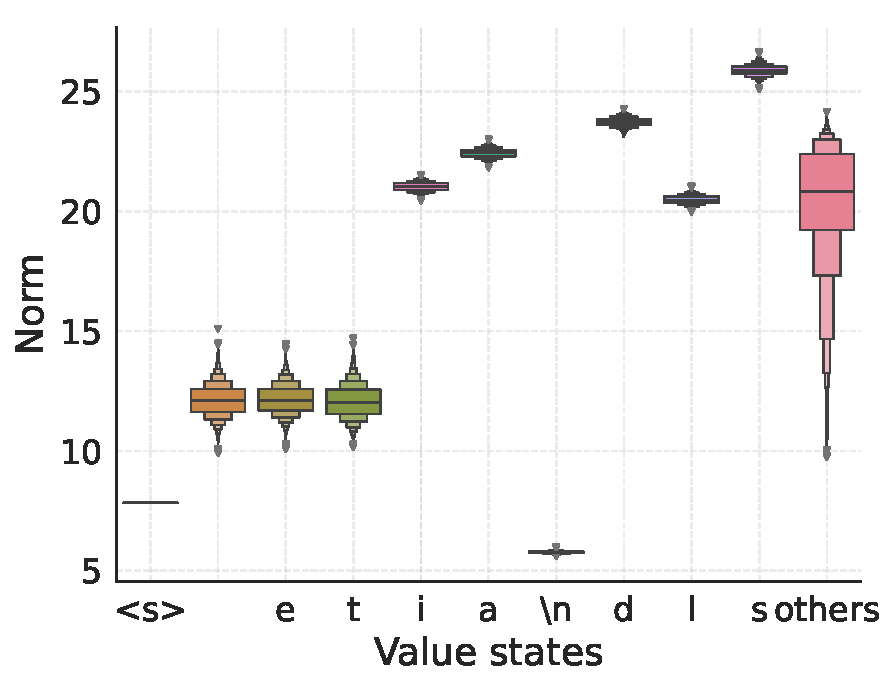
\includegraphics[width=\linewidth]{Figures/figures_pretraining/dormant_copy/dormant_copy_L3_minor.pdf}
  \end{minipage}
  \vspace{-1em}
  \caption{\small \textbf{The norms of hidden states in the dormant copy experiment} A summary of the norm distributions of the output of layer 1 (Figure \ref{fig:pretraining-massive-norm}) and the value states of layer 2 (Figure \ref{fig:pretraining-small-value}) in a 3-layer transformer trained on the \textit{dormant copy} task. The \bos~token is at the left most, with three trigger tokens ` ', `t', and `e' following it. We then randomly choose six tokens and separately summarize their norm distributions. We pull all other tokens together, forming the distribution of the norms of others at the right most. Only the \bos~and the $\backslash n$ token possess remarkably large output norms and small value states norms.}
  \label{figure:pretraining-findings-norms}
  \vspace{-1em}
\end{figure}

The inspection on the training dynamics enriches our understanding of the emergence of the dormant mechanism. Figure \ref{figure:pretraining-dynamics} summarises the change of multiple metrics along the training dynamics, including the ICL risk, the Markov prediction risk, the proportion of tokens that only attend to the \bos~token, the average attention weights on \bos, and the scaled norm of the output of layer 1 on \bos. Figure \ref{fig:pretraining-dynamics-long} presents their change along the entire training steps. The norm of the \bos~in layer 1 keeps increasing while other metrics remain unchanged. Figure \ref{figure:pretraining-dynamics} zooms in on the first 0 to 1000 steps along the training steps. The dynamics exhibit three phases: 1. Markov learning phase (0 to 140 steps): The prediction risk on normal tokens drops; the ICL risk firstly drops then stuck at a relatively high level; there is neither large attention weights nor massive output norms on the \bos~token. 2. ICL learning phase (140 to 240 steps): The prediction risk on normal tokens has negligible decrease; the ICL risk drops sharply; at the same time, the attention weights on the \bos~token increase and the output norms of \bos~slightly decreas. 3. Attention sink and massive norm formation phase (after 240 steps): the ICL risk decreases slowly and remains unchanged after 1000 training steps; the attention weights and the proportion of dormant tokens keep increasing; the output norm of \bos~keeps increasing along all training steps.

\begin{figure}[t]
\centering
    \begin{minipage}{0.4\textwidth}
      \centering
      \subcaption{\small From 0 to 10000 steps}
      \label{fig:pretraining-dynamics-long}
      \vspace{-.2em}
      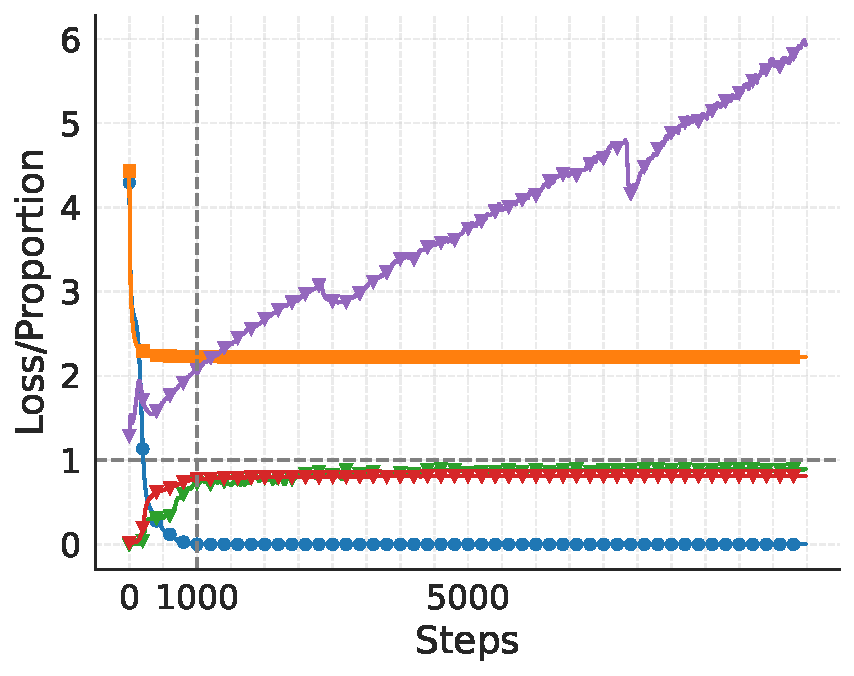
\includegraphics[width=\linewidth]{Figures/figures_pretraining/dormant_copy/dormant_copy_dynamics_long.pdf}
  \end{minipage}
    \begin{minipage}{0.4\textwidth}
      \centering
      \subcaption{\small Zoom in on 0 to 1000 steps}
      \label{fig:pretraining-dynamics}
      \vspace{-.2em}
      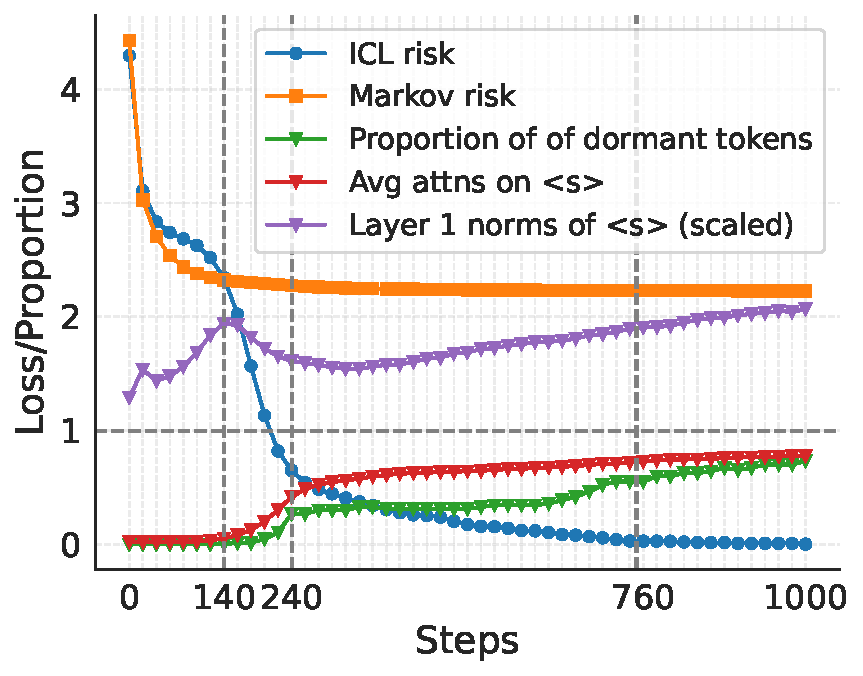
\includegraphics[width=\linewidth]{Figures/figures_pretraining/dormant_copy/dormant_copy_dynamics.pdf}
  \end{minipage}
  \hspace{-1em}

  \vspace{-1em}
  \caption{\small \textbf{Training dynamics of the dormant copy experiment} The ICL risk computes the prediction risk on trigger tokens; the Markov risk computes the prediction risk on normal tokens; we count the number of tokens that have attention weights on the \bos~token greater than 0.9 and get the proportion of dormant tokens; we take the average attention weights on \bos~from normal tokens; for better visualization and since only the trend is important in our message, we scale down the output norm of \bos~by $20$. The training dynamics possess three phases, with the Markov risk drops first, then the ICL risk together with the attention sink, and finally the massive norm emerges.}
  \label{figure:pretraining-dynamics}
  \vspace{-1em}
\end{figure}
